\chapter{Marco teórico y estado del arte}
\section{biologia}
\subsection{Microbiota}
La microbiota es el conjunto de microorganismos (bacterias, virus, arqueas, u hongos) que habitan en un ambiente, ya sea en organismos multicelulares como humanos~\cite{gilbert2018current}, animales~\cite{bahrndorff2016microbiome} o plantas~\cite{berendsen2012rhizosphere}, o en ambientes naturales como el océano~\cite{doi:10.1126/science.aac8455} o el suelo~\cite{banerjee2023soil}. Estos organismos presentes en la microbiota se encuentran en un estado de simbiosis junto con el host, contribuyendo en funciones vitales como la homeostasis, regulación del sistema inmune, digestión de alimentos, producción de vitaminas, protección ante enfermedades y agentes patógenos~\cite{marco2021defining,fijan2014microorganisms,altvecs2020interaction,hou2022microbiota}. Sin embargo, una disbiosis o una baja diversidad en la microbiota puede llevar a una desregulación del organismo, incluyendo diversos tipos de enfermedades, fallas en el sistema inmune, falta de vitaminas, trastornos como depresión, estrés, e incluso diferentes tipos de cáncer en el caso del ser humano~\cite{altvecs2020interaction,hou2022microbiota}.

La composición de la microbiota va cambiando dependiendo del área que se está colonizando, pudiéndose econtrar diferentes microorganismos en las cavidades orales, zonas intestinales, genitales, cutáneas o tracto respiratorio~\cite{ursell2012interpersonal}.

Se estima que en el ser humano habitan más de 10 billones de microorganismos~\cite{sender2016revised}, es decir, poseemos cerca de 350 billones de celulas microbioanas~\cite{fijan2014microorganisms,ley2006ecological} , siendo este número al menos 10 veces mayor que el número de células humanas que poseemos.

En la naturaleza los microorganismos cumplen un rol fundamental en los ciclos bioquímicos del nitrógeno, carbono y fósforo~\cite{bitton1994role, gougoulias2014role}, como también en los procesos de desnitrificación, nitrificación y mineralización~\cite{bitton1994role, gougoulias2014role}. 
Dependiendo del tipo de ambiente, los microorganismos también varian, en el caso del suelo por ejemplo, cambian dependiendo del tipo de suelo en el que están (agrícolas, forestales, humedales, pastos o suelos desérticos~\cite{jiao2021linking}) y de las características de éste como la temperatura, hidaratación, profundidad, cantidad de carbono~\cite{bickel2020soil}.
En el caso de las plantas, se ha demostrado, que la microbiota presente ayuda a la adquisición de nutrientes~\cite{hu2017probiotic}, al crecimiento, salud de las plantas y resistencia a enfermedaddes~\cite{lemanceau2017let,hardoim2015hidden,vorholt2012microbial,COMPANT201929}.


La microbiota humana se puede ver afectada por diferentes factores, como los hábitos alimenticios, estilo de vida, uso de antibióticos, la edad, estrés, entre otros~\cite{altvecs2020interaction}. La interacción con el medio ambiente influye notoriamente también, habiendo estudios que identifican cambios en la microbiota intestinal y cutánea en niños que interactuan con la naturaleza, plantas o suelo, identificando también un aumento de vías inmunoreguladoras en comunidades microbianas cercanas a la naturaleza~\cite{roslund2020biodiversity}. También se han identificado cambios en la microbiota de recién nacidos, infantes y adultos que viven con animales~\cite{tun2017exposure, azad2013infant,kates2020household}.


% https://www.frontiersin.org/articles/10.3389/fcimb.2012.00104/full?portfolio-raia-drogasil=1


% Microbiota: Microorganismos vivos encontrados en un ambiente definido (como por ejmplo en los tejidos orales o intestinales)

% microbioma: Colección de genomas de todos estos microorganismos en el ambiente (no solo las comunidades, elementos de su estructura microbial, metabolitos.)
Conocer la diversidad microbiana asociada a organismos multicelulares permite conocer microorganismos patógenos que causan enfermedades infecciosas,lo cual ayudaría al diagnóstico y permitiría tomar acciones oportunas~\cite{yan2018municipal,rackaityte2020human}. 

\subsection{ARN Ribosomal 16S}
El gen 16S rRNA es el marcador molecular más utilizado para la identificación de bacterias y comunidades microbianas~\cite{janda200716s,lopez2023determining}. Posee caracteristicas únicas, como su presencia en todas las bacterias, su alto grado de conservación (debido a que su función no cambia a través del tiempo) y su tamaño, el cuál permite ser lo suficientemente largo y preciso para la asignación taxónomica, y abordable para análisis bioinformáticos ~\cite{janda200716s, patel200116s}.

El gen 16S rRNA esta compuesto de aproximadamente 1542 pares de bases divididas en 10 regiones conservadas y 9 regiones hipervariables~\cite{clarridge2004impact}.%, las cuales permiten llevar a cabo la  identificación de los organismos. 
\begin{figure}[H]
    \centering
    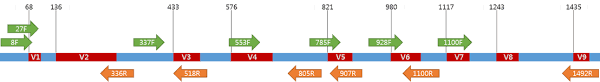
\includegraphics[width=1\linewidth]{images/16S.png}
    \caption{Estructura de las regiones variables e hipervariables del gen 16S rRNA}
    \label{fig:16S_structure}
\end{figure}
\begin{figure}[H]
    \centering
    \includegraphics[width=1\linewidth]{images/16S_2.png}
    \caption{Estructura de las regiones variables e hipervariables del gen 16S rRNA}
    \label{fig:16S_structure2}
\end{figure}

\hl{hacer denuevo la figura}

Las regiones hipervariables permiten llevar a cabo la caracterización de los microorganismos. Diversos estudios se han llevado a cabo para determinar los efectos de la selección de la región a utilizar para la identificación, llegandose a determinar que la región hipervariable ha utilizar influye en los resultados de la comunidad y en la diversidad de organismos que se caracteriza~\cite{klindworth2013evaluation,mizrahi2013taxonomic,guo2013taxonomic,soergel2012selection}, y también que ciertas regiones hipervariables permiten identificar mejor ciertos grupos taxonómicos~\cite{buscar}.

%\hl{Evaluation of general 16S ribosomal RNA gene PCR primers for classical and next-generation sequencing-based diversity studies} \hl{The impact of DNA polymerase and number of rounds of amplification in PCR on 16S rRNA gene sequence data, mSphere, vol. 4, 2019}



Con el desarrollo de las tecnologías de secuenciación masiva, su bajo costo y alto througput, la forma de caracterizar bacterias se ha vuelto más estándar y abordable al día de hoy~\cite{woo2008then, tanner1994impact}. El estudio de comunidades microbianas mediante el gen 16S rRNA se ha vuelto una herramienta poderosa tanto en ambientes clínicos, como ambientales, \hl{incluso llegandose a secuenciar en el espacio}, permite obtener información de la diversidad de una muestra de manera mucho más rápida y económica que los métodos tradicionales~\cite{buscar}.
%Las tecnologías de secuenciación  permiten la identificación de bacterias a través de  \hl{signatures/firmas} únicas 
\subsection{Secuenciación de ADN}

\hl{que es la secuenciaciónd de adn}
Mediante la secuencación de ADN se puede caracterizar genomas completos, 


Con la aparición de las tecnologías de secuenciación de segunda y tercera generación~\cite{janda200716s,pollock2018madness}, la secuenciación del gen 16S rRNA se convirtió en es una técnica masiva hoy en día para la caracterización de comunidades microbioanas e identificación tanto de patogenos o aislamiento de bacterias clínicas~\cite{patel200116s}.

Estos métodos requieren la amplificación y secuenciación del gen 16S rRNA y el uso de herramientas biofinformáticas para la identificación y comparación con bases de datos.

Con la secuenciación del gen 16S rRNA se obtiene un conjunto de lecturas de ADN, donde cada lectura pertenece a una bacteria presente en la muestra. Estas lecturas se procesan y se comparán con bases de datos existentes para poder realizar la asignación taxonómica y poder identificar la bacteria. Finalmente lo que se obtiene es un perfil de toda la comunidad bacteriana de la muestra, todas las bacterias presentes que las herramientas bioinformáticas pudieron detectar, junto con su abundancia relativa.

Existen diferentes tecnologías de secuenciación cada una de ellas con diferentes largos de las lecturas a secuenciar,diferente porcentaje de error, costo y througput. Cada una de ellas tiene sus ventajas y desventajas, y los análisis bioinformáticos a realizar cambian dependiendo de la tecnología a utilizar~\cite{bierman2014understanding}.
La precisión de estas tecnologías se puede medir mediante la precisión de la lectura raw (precisión al leer un sólo fragmento de ácido nucleico a la vez) o la precisión de los ensamblajes mediante consensos (reconstrucción de genomas completos ) 

El umbral para distinguir especies bacterianas utilizando el gen 16S rRNA es de mínimo 97\% de similitud~\cite{kim2014towards}
\hl{LEEER} https://www.microbiologyresearch.org/content/journal/ijsem/10.1099/ijs.0.059774-0


diversidad, riquesa y composición de la comunidad microbiana
\subsubsection{Sanger}
Incialmente el gen 16S completo se seucenciaba mediante sanger ~\cite{sanger1975rapid} pero debido a su alto costo y complejidad de llevar a cabo en laboratorio
\subsubsection{Illumina}
\hl{como funciona illumina}
Ultra-high-throughput microbial community analysis on the Illumina HiSeq and MiSeq platforms
Las tecnologías de secuenciación de segunda generación, como Illumina e IonTorrent permiten secuenciar solo una parte del gen 16S rRNA, debido a que las lecturas son cortas (300-400pb)~\cite{salipante2014performance}. Esto conlleva a que se deba decidir que región del gen secuenciar, para poder obtener la mayor diversidad posible presente en la muestra. Diversos estudios se han realizado para analizar que región permite obtener esta diversidad de manera precisa~\cite{liu2008accurate,schloss2011reducing}, llegando a descubrirse que ciertos grupos taxonómicos se identifican de mejor manera al utilizar cierta regiones hipervariables~\cite{he2013comparison,claesson2010comparison}.

Illumina se ha convertido hoy en día en el estándar más utilizado para la secuenciación del gen 16S debido a su bajo costo, alta precisión (99.9\%) y througput~\cite{pichler201816s}. Sin embargo, esta tecnología esta limitada por el largo de las lecturas, debido a que al secuenciar con illumina solo se puede secuenciar una o dos regiones del gen 16S (de las 9 regiones hipervariables), lo que límita la resolución taxónomica, permitiendo asignar correctamente solo a nivel de genero~\cite{johnson2019evaluation}

Existen diferentes metodologías pensadas para trabajar con illumina,debido a que se sabe que existe presencia de ruido, como la eliminación de quimeras, la eliminación de singleton y otus raros son recomendasos~\cite{caporaso2011global,auer2017analysis}, realizar denoising con dada~\cite{callahan2016dada2} y unoise~\cite{edgar2016unoise2}, pero todas estas metodologías no esgtan disponibles para usarse con annopore, debido al porcentaje de error y al secuenciar todo el gen 16s.
Mientras algunos estudios han demostrado, que Nanopore presenta un porcentaje de ruido muy bajo, casi nulo~\cite{szoboszlay2023nanopore}, y a su vez, al secuenciar el gen completo, y no contar con OTUs, o ASV, permite mejorar el rendimiento de los estimadores de riqueza que se basan en estas metodologias, como los índices de chao1~\cite{chao1984nonparametric}, ACE~\cite{chao1992estimating}, o brakaway~\cite{willis2015estimating}


Illumina sobrerepresenta el numero de especies debido al ruido? \hl{Nanopore is preferable over ...}

Es por esto, que las tecnologías de tercera generación como Oxford Nanopore y PacBio se presentan como opciones prometedoras para la secuenciación del gen 16S rRNA, debido a su bajo costo y su capacidad de secuenciar el gen completo en una sola lectura, lo que permite una mayor resolución taxonómica a nivel de especie o incluso de strain~\cite{szoboszlay2023nanopore}~\cite{urban2021freshwater,delahaye2021sequencing}. \hl{revisar estas citas}

% \hl{ESTOY VIENDO ACA } https://www.mdpi.com/2076-2607/11/3/804#B1-microorganisms-11-00804
\subsubsection{Oxford Nanopore}
Debido a su capacidad de secuenciar lecturas desde unas pocas kilobases hasta megabases~\cite{amarasinghe2020opportunities}, permite obtener información genómica más completa y contigua que las tecnologías de secuenciación de segunda generación, como Illumina.

Su bajo costo y su portabilidad, que permiten secuenciar 

En sus inicios, la mayor limitante de utilizar Oxford Nanopore era su alto porcentaje de error. En el 2019 estudios reportaban que llegar a una resolución de especie no era aún posible con Nanopore~\cite{winand2019targeting}. Estudios posteriores, determinaron que la precisión de secuenciación se encontraba entre el 92\% al cerca del 96\%~\cite{urban2021freshwater,delahaye2021sequencing}, siendo aún inviable para la asignación taxonómica a nivel de especie \hl{creo que deberia tener cuidado con esto, ya que este paper lo dice, pero otros no}. Sin embargo, con la introducción de la nueva química a finales del 2021, el porcentaje de error reportado por nanopore disminuye notablemente, llegando a un 99.9\% de precisión, permitiendo la resolución taxónomica de especie~\cite{yoon2017introducing}.\hl{buscar más citas}


\section{Herramientas}
\subsection{Asignación taxónomica}
Existen diferentes herramientas para hacer asignación taxonómica de secuencias, algunas incluyen una asignación taxonómica directa a los datos luego del control de calidad, mientras otras herramientas buscan minimizar el error de Oxford Nanopore mediante metodologías de clustering o de algoritmos de maximización de expectativas. Algunas de las más utilizadas para datos de Oxford Nanopore se presentan a continuación:

\hl{es posible ponerle numeritos a las subsubsection?}

Hoy en día no hay establecidas buenas practicas para el procesamiento del gen 16S rRNA secuenciado mediante Oxford Nanopore, tanto al hablar de la herramienta para hacer asignación taxonómica, como al hablar de la base de datos al utilizar.\hl{leer para ver si citar https://academic.oup.com/femsec/article/97/3/fiab001/6098400}
\subsubsection{Epi2me}
Plataforma desarrollada por Oxford Nanopore para el análisis de datos secuenciación obtenidos mediante sus dispositivos. 
Integra flujos de trabajo para realizar basecalling y demultiplexación, alineamiento, ensamblaje de SARS-CoV-2, asignación taxonómica de gen 16S, 18S, ITS, y metagenómca, variant calling, entre otros.

Mediante la interfaz gráfica el usuario puede seleccionar el análisis a realizar y configurar los parámetros. Debido a su interfaz de fácil uso permite al usuario abstraerse de la ejecución de herramientas o flujos de trabajo y de la necesidad de contar con recursos computacionales para la ejecución de los mismos.
Los resultados se pueden descargar y visualizar mediante la misma plataforma.
%solo requiere acceso a internet por lo que es una buena alternativa para usuarios que no cuentan con recursos computacionales para el analisis de datos de secuenciacion. Sin embargo, la mayoria de sus flujos de trabajo solo cuenta con análisis primarios y no permite la personalización de los scripts o procesos realizados por lo que en caso de requerir una solución personalizada no se podría llevar a cabo mediante la plataforma. De igual manera, al contar solo con analisis primarios, los analisis posteriores deben ser realizados por el usuario mediante el uso de otras herramientas. 


Para la asignación taxónomica del gen 16S utiliza la herramienta blast con la base de datos de Genbank.

% \begin{itemize}
%     \item Qscore mínimo: 7
%     \item Longitud de lectura mínima: 0
%     \item Longitud de lectura máxima: 0
%     \item e-value máximo: 0.01
%     \item coverage mínimo: 30\%
%     \item Porcentaje de identidad mínimo: 77\%
%     \item max target sequences:
% \end{itemize}
El output de esta herramienta es un archivo en formato CSV con la información de la lectura, asignación taxonómica a nivel de especie, porcentaje de identidad de la asignación, entre otras.
\subsubsection{NanoCLUST}
Nanoclust~\cite{10.1093/bioinformatics/btaa900} es un flujo de trabajo desarrollado en Nextflow para la clasificación de amplicones del gen 16s obtenidos mediante secuenciación de Oxford Nanopore. Incluye pasos previos a la asignación taxonomica, como el basecalling, demultiplexación y control de calidad. Destaca por utilizar un clustering no supervisado (UMAP) y un paso exhaustivo de corrección de lecturas basada en los clusters obtenidos previo a la asignación taxonómica.
Utiliza la base de datos de Genbank para realizar la asignación taxonómica.

Cabe destacar que este flujo de trabajo se encuentra descontinuado ya que fue desarrollado utiilzando Nextflow DSL1 (estándar deprecado en la version 22.10.x). Además, debido a que la herramienta ha dejado de recibir soporte por parte de los desarrolladores, no se han actualizado pasos claves, como el basecalling y demultiplexación (pasos opcionales).

El output de esta herramienta es un archivo csv por cada categoría taxonómica (filo, clase, orden, familia, género, especie) con la cantidad de lecturas asignadas a cada taxonomía. De igual forma, se generan graficos de barra con las asignaciones, y un gráfico de la separación de los clusters. \hl{mejorar}. 
\subsubsection{NanoRTax}

NanoRTax~\cite{RODRIGUEZPEREZ20225350} es un flujo de trabajo desarrollado en Nextflow que cuenta con una interfaz web que permite al usuario visualizar el progreso y resultados del pipeline.
Recibe como entrada los archivos FASTQ, a los cuales se les hace un control de calidad mediante fastp, y a continuación se realiza la asignación taxonómica mediante las herramientas Kraken2, Centrifuge y BLAST. 

Al igual que NanoCLUST, NanoRTax utiliza DSL1 por lo que no es comptabile con versiones nuevas de Nextflow.

El output de esta herramienta \hl{XX}
\subsubsection{EMU}
EMU~\cite{curry2022emu} busca realizar una corrección de errores y mejorar el error de Oxford Nanopore mediante un enfoque basado en algoritmos de maximización de expectativas para generar perfiles taxonómicos de la comunidad microbiona. Permite realizar estos perfiles utilizando diferentes bases de datos, como, la base de datos de Genbank,  RDP y Silva v.138. En el caso de realizar analisis de la región ITS, permite integrar las base de datos de UNITE de fungi y eucariotas.

El output de esta herramienta es un archivo en formato TSV con los perfiles taxonómicos encontrados en cada muestra, es decir, el identificador del taxón, abundancia, especie y la información de todas las categorías taxonómicas. 

\subsubsection{EzBioCloud Microbial Taxonomic Profiling (MTP) pipeline and the PKSSU4.0 database}
En algunos estudios se ha utilizado % https://www.mdpi.com/2076-2607/11/3/804#B1-microorganisms-11-00804 , 
\subsubsection{VSEARCH [35] against the EzBioCloud 16S database.?}
\subsection{Herramientas bioinformáticas}
Existen diferentes herramientas bioinformáticas que se pueden utilizar para el análisis y manipulación de datos de secuenciación, a continuación se presentan algunas de las más relevantes para este trabajo:

\subsubsection{Guppy}
Guppy es una suite de herramientas provista por Oxford Nanopore para realizar procesamientos de datos de secuenciación básicos. Permite realizar basecalling y demultiplexación, alineamiento, detección de bases modificadas, etc.
\subsubsection{FastQC}
FastQC\cite{andrews2010fastqc} permite visualizar la calidad de los datos mediante métricas estándar de calidad, contenido GC, distribución de tamaños, niveles de duplicación  y contenido de adaptadores.


Genera un reporte en formato html de fácil visualización separado por módulos, donde cada módulo presenta un estado de Aprobado, Fallido o Advertencia (dependiendo de la calidad de los datos). Se desarrollo pensando en tecnología de secuenciación de lecturas cortas, las cuales poseen un porcentaje de error mucho más bajo que las tecnologías de secuenciación de tercera generación y en análisis de genoma completo, por lo que algunos módulos pueden mostrarse como fallidos debido a la naturaleza de los datos de Oxford Nanopore, sin ser datos de baja calidad.
\subsubsection{NanoPlot}
NanoPlot~\cite{10.1093/bioinformatics/btad311} es una herramienta para la evaluación de calidad de datos de secuenciación de lecturas largas, permite visualizar la información de calidad, largo de lecturas y distribución de estas mediantes gráficos interactivos.

Genera un reporte en formato html y gráficos interáctivos que permiten visualizar la calidad de los datos, longitud de las lecturas, distribución de la calidad y longitud, entre otros.
\subsubsection{Fastp}

Fastp\cite{chen2018fastp} es una herramienta de alto rendimiento diseñada para el procesamiento de archivos fastq, permite realizar filtrado de secuencias (por calidad, largo), recortar extremos de baja calidad, recortar adaptadores, eliminar colas polyA, etc.
\subsubsection{MultiQC}
MultiQC \cite{ewels2016multiqc} es una herramienta que permite resumir la información obtenida por diferentes herramientas bioinformaticas en un solo informe final. También permite integrar varias muestras en un solo reporte, y multiples pasos de analisis en un solo archivo html.

% Permite una visualización interactiva de los graficos, mediante la cual se puede hacer zoom o quitar muestras de los 
\subsubsection{PICRUSt2}
PICRUSt2~\cite{douglas2020picrust2} es una herramienta para la predicción funcional utilizando secuencias marcadoras de genes.
Generalmente se utiliza el gen 16S rRNApara realizar la predicción, pero también se pueden usar otros genes marcadores.

El output entrega archivos en formato CSV con la abundancia de los genes ortologos, la clasificación de las enzimas y las vías metabolicas predichos en cada muestra.

\subsubsection{LEfSe}
LEfSe (Linear discriminant analysis Effect Size)~\cite{segata2011metagenomic}  determina las caracteristicas que permiten explicar las diferencias entre diferentes clases o grupos al combinar pruebas estándar de significancia estadistica junto con pruebas que codifican la consistencia biologica y relevancia del efecto encontrado. 
\subsubsection{vegan package}
Vegan~\cite{dixon2003vegan} es un paquete desarrollado para R que permite realizar análisis de la ecología comunitaria descriptiva. Contiene funciones de análisis de diversidad,  metodos de ordenación comunitaria, análisis de disimilitud, funciones para vegetación y ecologos comunitarios.

% Tiene como objetivo el desarrollo 


\subsubsection{Taxonkit}
Taxonkit~\cite{SHEN2021844} permite la manipulación de información taxónomica de NCBI de una manera comprensiva y eficiente. Dado un identificador taxonómico o un nombre de especie se puede obtener el linage completo de esta.

\subsubsection{csvtk}
csvtk es una herramienta multiplataforma, eficiente y practica para la manipulación de archivos en formato CSV y TSV. Esta herramienta esta desarrollada para utilizarse en conjunto con otras suites de herramientas como TaxonKit, permitiendo obtener resultados de taxonómia de fácil visualización y manipulación para la integración en flujos de trabajo o scripts.
\subsubsection{NCBI database}
Tanto EPI2ME como Nanoclust utilizan la base de datos de ncbi.
\subsection{Lenguajes de programación y Frameworks}
\subsubsection{Nextflow}
Nextflow~\cite{di2017nextflow} es un framework open source para el desarrollo de flujos de trabajo, el cual permite la ejecución de éstos en diferentes entornos computacionales, ya sea en un computador personal, una plataforma de cómputo de alto rendimiento o en la nube. También permite la ejecución de flujos de trabajo de manera paralela, manejando los recursos computacionales de manera eficiente, y sencilla para el usuario.
 Al permitir el desarrollo de flujos de trabajo escalables y reproducibles es una buena alternativa que ha ganado popularidad debido a su facilidad de uso.

Cuenta con una comunidad llamada nf-core que se encarga de desarrollar flujos de trabajo para el análisis de datos biologicos, los cuales son revisados por la comunidad y publicados en su repositorio. Esto permite contar con una gran cantidad de flujos de trabajo disponibles, los cuales pueden ser ejecutados de manera sencilla por los usuarios, pero cabe destacar que hay que tener conocimientos de linea de comando para poder ejecutarlos.


\subsubsection{python?}
\subsubsection{js}

\subsubsection{r?}

\subsubsection{FastAPI}
Framework rápido  y ligero para el desarrollo de APIs modernas de manera ágil utilizando Python y basado en sus anotaciones de tipo estandar.
Utiliza pydantic para la validación de los datos de entrada y salida y starlette para el manejo de las peticiones HTTP. \hl{no estoy 100\% segura}
\subsubsection{SQLalchemy}
ORM (Object-Relational Mapping) para Python que permite la comunicación entre el back end y la base de datos SQL de manera sencilla, transformando los resultados de la base de datos en estructuras utilizables mediante Python. Gestiona la creación de modelos y consultas de forma sencilla.
\subsubsection{Vue.js}
Vue es un framework para la construcción de interfaces de usuario. Se basa en JavaScript, HTML y CSS para proporcionar un modelo de programación declarativo y basado en componentes que permite desarrollar interfaces de manera eficiente.
\subsubsection{TypeScript}
TypeScript~\cite{bierman2014understanding} es un lenguaje de programación basado en JavaScript, el cual añade sintaxis adicional a JavaScript (o frameworks basados en JS) para soportar la integración de tipado de datos. Al especificar los tipos de datos, TypeScript tiene la capacidad de validarlos e informar errores cuando estos no correspondan.
\subsubsection{Vuetify}
Vuetify es un proyecto de código abierto para la construcción de interfaces utilizando los componentes de Vue. Permite la personalización de los componentes con SASS y SCSS, cuenta con un diseño responsivo, y una gran cantidad de componentes ya predefinidos.
\subsubsection{PostgreSQL}
PostgreSQL es un sistema de gestión de bases de datos relacionales de código abierto basado en POSTGRES. Permite el uso de tipos de datos complejos realizar consultas tanto relacionales (SQL) y no relacionales (JSON).

\subsection{Gestores de paquetes}
\subsubsection{Conda}
Conda~\cite{anaconda}  es una herramienta de código abierto, multiplataforma  que permite la gestión de paquetes, dependencias y entornos de desarrollo de manera sencilla. Permite aislar entornos virtuales con caracteristicas especificas, lo que facilita la reproducibilidad de los análisis y la portabilidad de los mismos. \hl{já}
\subsubsection{Apptainer}
Apptainer (antes llamado Singularity~\cite{kurtzer2017singularity}) simplifica la creación y ejecución de contenedores, asegurando el encapsulamiento de los componentes de softwares necesarios para su reproducibilidad y portabilidad.  
\subsubsection{Docker}
\hl{Creo que no es necesario}

\subsection{Métricas para la evaluación de la diversidad microbiana}
La diversidad microbiana 

Los índices de diversidad se dividen en índices de riqueza o uniformidad/divergencia
\subsubsection{Indice de simpson}
\subsubsection{Indice de shannon}
\subsubsection{Indice de chao2}

